\documentclass[serif]{beamer}\usepackage[]{graphicx}\usepackage[]{color}
%% maxwidth is the original width if it is less than linewidth
%% otherwise use linewidth (to make sure the graphics do not exceed the margin)
\makeatletter
\def\maxwidth{ %
  \ifdim\Gin@nat@width>\linewidth
    \linewidth
  \else
    \Gin@nat@width
  \fi
}
\makeatother

\definecolor{fgcolor}{rgb}{0.345, 0.345, 0.345}
\newcommand{\hlnum}[1]{\textcolor[rgb]{0.686,0.059,0.569}{#1}}%
\newcommand{\hlstr}[1]{\textcolor[rgb]{0.192,0.494,0.8}{#1}}%
\newcommand{\hlcom}[1]{\textcolor[rgb]{0.678,0.584,0.686}{\textit{#1}}}%
\newcommand{\hlopt}[1]{\textcolor[rgb]{0,0,0}{#1}}%
\newcommand{\hlstd}[1]{\textcolor[rgb]{0.345,0.345,0.345}{#1}}%
\newcommand{\hlkwa}[1]{\textcolor[rgb]{0.161,0.373,0.58}{\textbf{#1}}}%
\newcommand{\hlkwb}[1]{\textcolor[rgb]{0.69,0.353,0.396}{#1}}%
\newcommand{\hlkwc}[1]{\textcolor[rgb]{0.333,0.667,0.333}{#1}}%
\newcommand{\hlkwd}[1]{\textcolor[rgb]{0.737,0.353,0.396}{\textbf{#1}}}%
\let\hlipl\hlkwb

\usepackage{framed}
\makeatletter
\newenvironment{kframe}{%
 \def\at@end@of@kframe{}%
 \ifinner\ifhmode%
  \def\at@end@of@kframe{\end{minipage}}%
  \begin{minipage}{\columnwidth}%
 \fi\fi%
 \def\FrameCommand##1{\hskip\@totalleftmargin \hskip-\fboxsep
 \colorbox{shadecolor}{##1}\hskip-\fboxsep
     % There is no \\@totalrightmargin, so:
     \hskip-\linewidth \hskip-\@totalleftmargin \hskip\columnwidth}%
 \MakeFramed {\advance\hsize-\width
   \@totalleftmargin\z@ \linewidth\hsize
   \@setminipage}}%
 {\par\unskip\endMakeFramed%
 \at@end@of@kframe}
\makeatother

\definecolor{shadecolor}{rgb}{.97, .97, .97}
\definecolor{messagecolor}{rgb}{0, 0, 0}
\definecolor{warningcolor}{rgb}{1, 0, 1}
\definecolor{errorcolor}{rgb}{1, 0, 0}
\newenvironment{knitrout}{}{} % an empty environment to be redefined in TeX

\usepackage{alltt}
\usetheme{Boadilla}
\usepackage{graphicx}
\usepackage[final]{animate}
\usepackage{breqn}
\usepackage{xcolor}
\usepackage{booktabs}
\usepackage{tikz}
\usetikzlibrary{decorations.pathreplacing}
\usetikzlibrary{shapes,arrows,positioning,shadows}
\usepackage{subfig}
\usepackage{pgf}

% change format of enumerated lists
\setbeamertemplate{enumerate items}[default]

\setbeamertemplate{navigation symbols}{}

% custom colors
\definecolor{mypal1}{HTML}{F0F9E8}\definecolor{mypal2}{HTML}{BAE4BC}\definecolor{mypal3}{HTML}{7BCCC4}\definecolor{mypal4}{HTML}{43A2CA}\definecolor{mypal5}{HTML}{0868AC}

\tikzstyle{decision} = [diamond, draw, text width=6em, text badly centered, inner sep = 2pt, top color=white, bottom color=mypal3, drop shadow]
\tikzstyle{block} = [rectangle, draw, text width=10em, text centered, rounded corners, minimum height=3em, minimum width=8em, top color = white, bottom color=mypal4,  drop shadow]
\tikzstyle{declare} = [rectangle, draw, text width=10em, text centered, minimum height=3em, minimum width=8em, top color = white, bottom color=mypal5,  drop shadow]

% knitr setup


% dependent data


% get online bib file


% my custom ggplot theme


% figure used on title page


\setbeamercolor{title}{fg=mypal5} % main title
\setbeamercolor{frametitle}{fg=mypal4, bg=mypal2} % frame titles
\setbeamercolor{structure}{fg=mypal4} % bottom banner
\setbeamercolor{normal text}{fg=mypal5}
\usebackgroundtemplate{
\includegraphics[height=\paperheight,width=\paperwidth]{fig/back_tmp.pdf}}

% macros
\newcommand{\emtxt}[1]{\textbf{\textit{#1}}}
\newcommand{\ShowSexpr}[1]{\texttt{{\char`\\}Sexpr\{#1\}}}
\newcommand{\Bigtxt}[1]{\textbf{\textit{#1}}}
\IfFileExists{upquote.sty}{\usepackage{upquote}}{}
\begin{document}

\title[Evaluating water quality]{\textbf{Quantitative approaches for biological assessment: Examples from Minnesota Lakes to Florida Estuaries}}
\author[M. Beck]{Marcus W. Beck, Ph.D.}

\institute[USEPA]{USEPA National Health and Environmental Effects Research Laboratory, Gulf Ecology Division, \href{mailto:beck.marcus@epa.gov}{beck.marcus@epa.gov}, Phone: 8509342480}

\date{May 22, 2017}

\titlegraphic{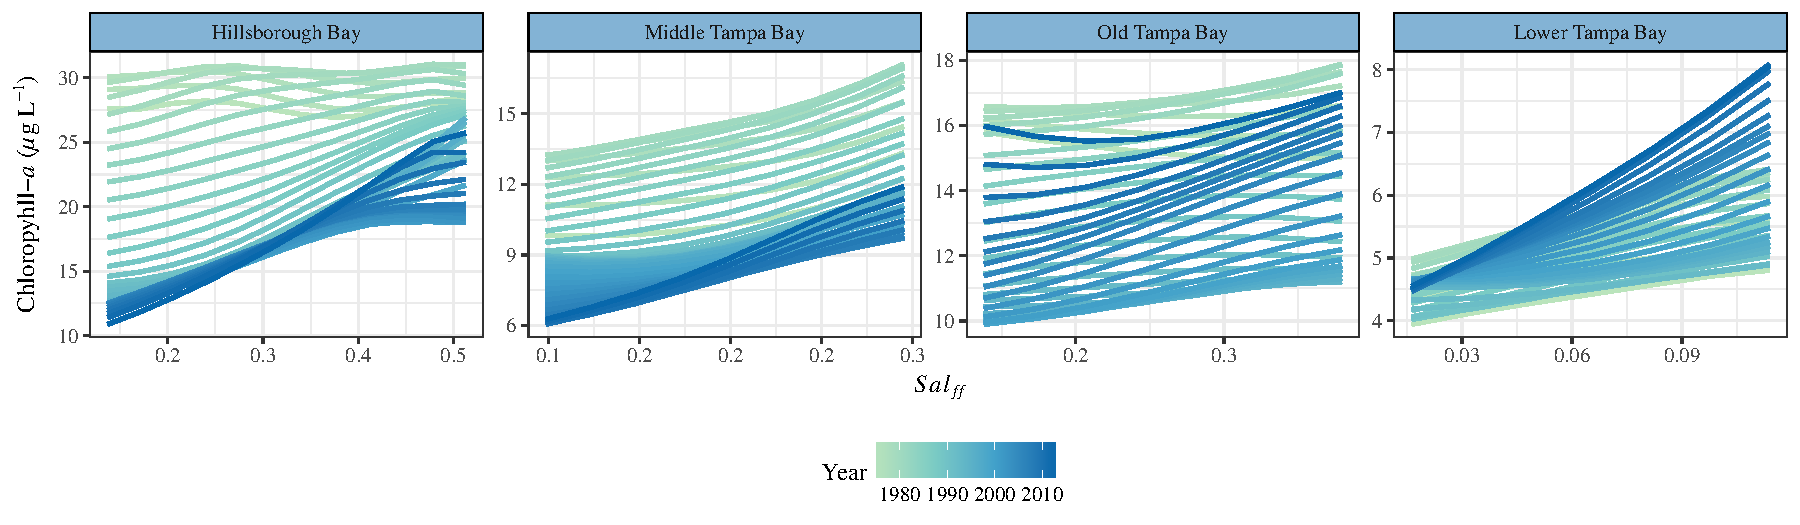
\includegraphics[width=0.95\linewidth]{fig/title_plo.pdf}}

%%%%%%
\begin{frame}[shrink]
\titlepage
\end{frame}

\section{Background}

%%%%%%
\begin{frame}{\textbf{Assessing environmental condition}}{\textbf{How do we collect and use data?}}
\onslide<+->
The foundation of environmental management is a strong monitoring network \scriptsize \cite{NRC90}\\~\\
\normalsize
Monitoring provides information for decision-making based on apparent trends...
\vspace{0.2in}
\begin{center}
\emtxt{What are the changes in environmental condition over time?}\\~\\
\emtxt{Are these changes `good' or `bad' based on our management objectives?}\\~\\
\emtxt{What may have caused these changes?}
\end{center}
\end{frame}

%%%%%%
\begin{frame}{\textbf{Assessing environmental condition}}{\textbf{How do we collect and use data?}}
\onslide<+->
\emtxt{The good news}: We are getting better at monitoring - standardized, automated, increased coverage, real-time/continuous \\~\\
\emtxt{The bad news}: Our ability to use these data for decision-making has not kept pace with availability! \\~\\
\onslide<+->


{\centering 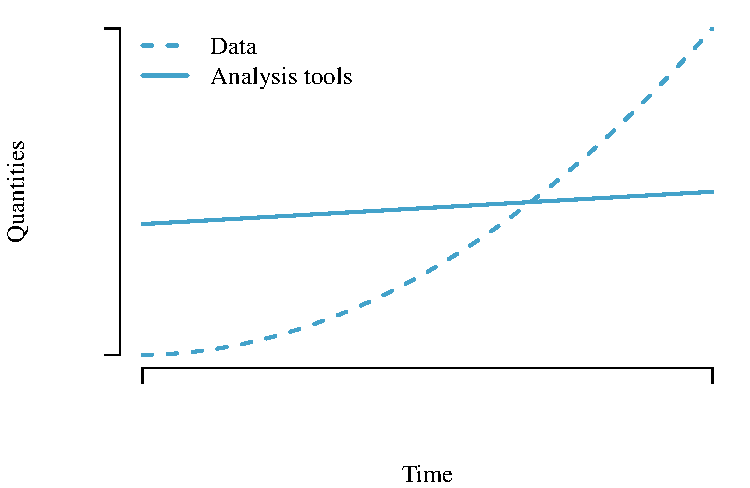
\includegraphics[width=0.55\textwidth]{fig/theo-1} 

}



\end{frame}

%%%%%%
\begin{frame}{\textbf{Assessing environmental condition}}{\textbf{How do we collect and use data?}}
\onslide<+->
Today's talk: My experience using environmental data to understand causes and dynamics of water quality change\\~\\
\begin{itemize}
\item \emtxt{Case 1}: Developing and quantifying response of a biotic index for Minnesota lakes \\~\\
\item \emtxt{Case 2}: Describing historical changes in eutrophication from long-term datasets in Tampa Bay \\~\\
\end{itemize}
\onslide<+->
Each case addresses the challenges of \emtxt{evaluating change} with biological endpoints and \emtxt{developing quantitative tools} to improve efficiency and understanding
\end{frame}

\section{Case 1: Minnesota lakes}

%%%%%%
\begin{frame}{\textbf{Case 1: Minnesota lakes}}{\textbf{Evaluating biological response}}
\begin{columns}
\begin{column}{0.5\textwidth}
\centerline{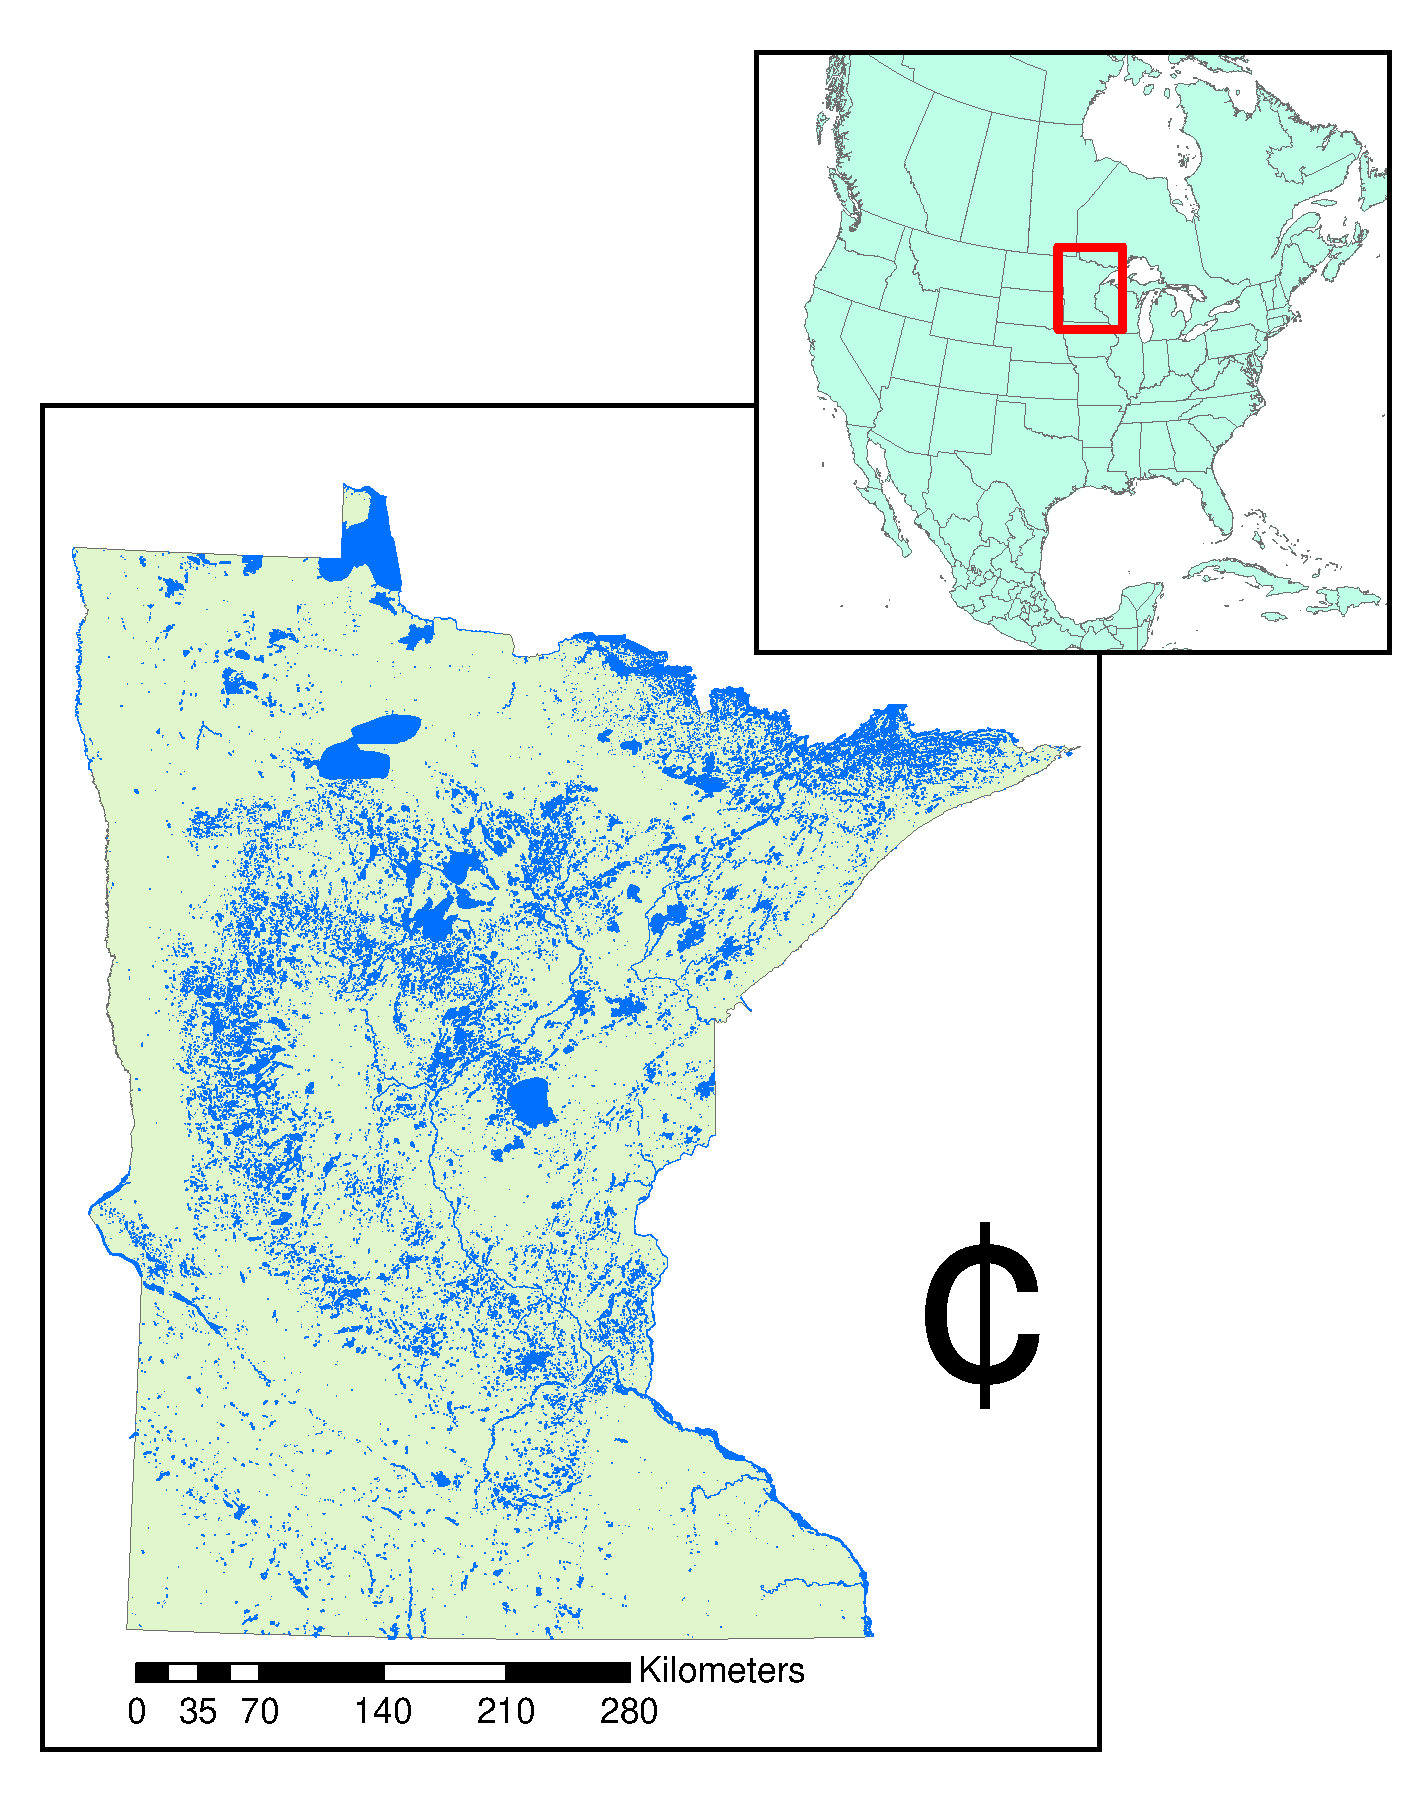
\includegraphics[width=\textwidth]{fig/mn_lake_inset.pdf}}
\end{column}
\begin{column}{0.5\textwidth}
\begin{center}

\includegraphics[width=0.5\textwidth]{fig/mn_seal.jpg} \\~\\
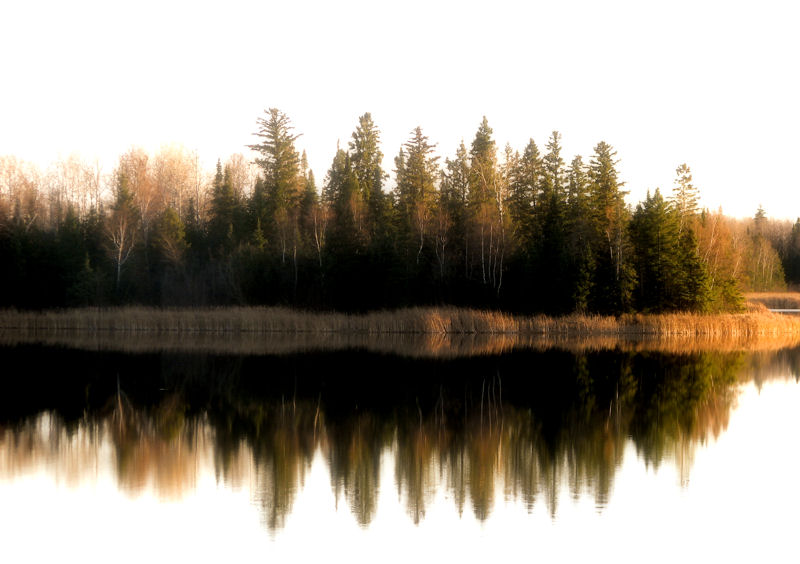
\includegraphics[width=0.8\textwidth]{fig/mn_lake.jpg}
\end{center}
\end{column}
\end{columns}
\end{frame}

% %%%%%%
% \begin{frame}{\textbf{Case 1: Minnesota lakes}}{\textbf{Evaluating biological response}}
% \onslide<+->
% Water Quality Act Amendments of 1972
% \begin{itemize}
% \item{Federal mandates to protect and restore the chemical, physical, and \emtxt{biological} integrity of surface waters}
% \item{Protection and restoration requires monitoring \\~\\}
% \end{itemize}
% \onslide<+->
% Index of biotic integrity (IBI) \cite{Karr81,Karr86}
% \begin{itemize}
% \item{Monitoring framework for definition and evaluation of biotic integrity}
% \item{Uses aquatic organisms as indicators of ecosystem health}
% \item{A multimetric index that is regionally specific}
% \end{itemize}
% \end{frame}

%%%%%%
\begin{frame}{\textbf{Case 1: Minnesota lakes}}{\textbf{Evaluating biological response}}
\onslide<+->
The macrophyte IBI can be used to evaluate relative lake condition by monitoring and evaluating aquatic plant metrics \cite{Beck10,Beck13} \\~\\
\onslide<+->
Includes eight metrics, summed to get one IBI score per lake \\~\\
\begin{itemize}
\item{MAXD: Maximum depth of plant growth}
\item{LITT: Percentage of littoral zone vegetated}
\item{OVER: Number of species with frequency occurrence $>$10\%}
\item{EMFL: Relative frequency of emergent-floating species}
\item{SUBM: Relative frequency of submersed species}
\item{SENS: Relative frequency of sensitive species}
\item{TOLR: Relative frequency of tolerant species}
\item{TAXA: Number of native taxa \\~\\}
\end{itemize}
\end{frame}

%%%%%%
\begin{frame}{\textbf{Case 1: Minnesota lakes}}{\textbf{Evaluating biological response}}
\begin{columns}
\onslide<+->
\begin{column}{0.5\textwidth}
\begin{center}
Related to changes in water quality \\~\\
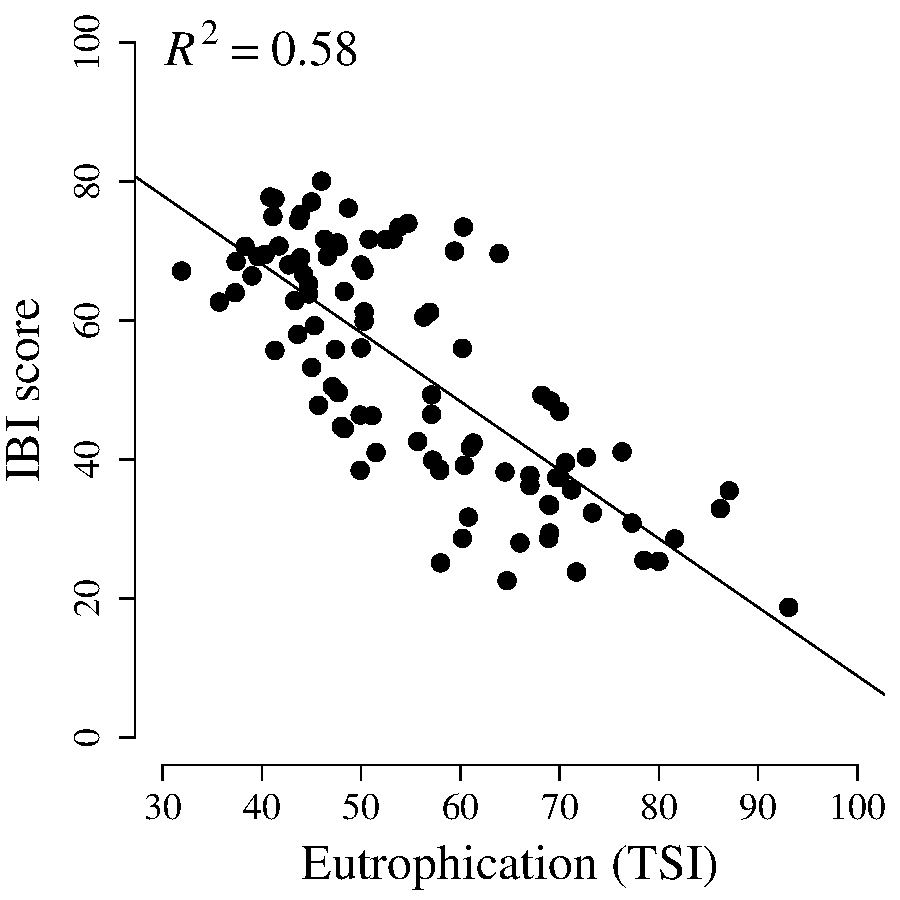
\includegraphics[width=\textwidth]{fig/Beck_GEDsem-ibi_tsi.pdf}
\end{center}
\end{column}
\onslide<+->
\begin{column}{0.5\textwidth}
\begin{center}
High precision given sampling effort \\~\\
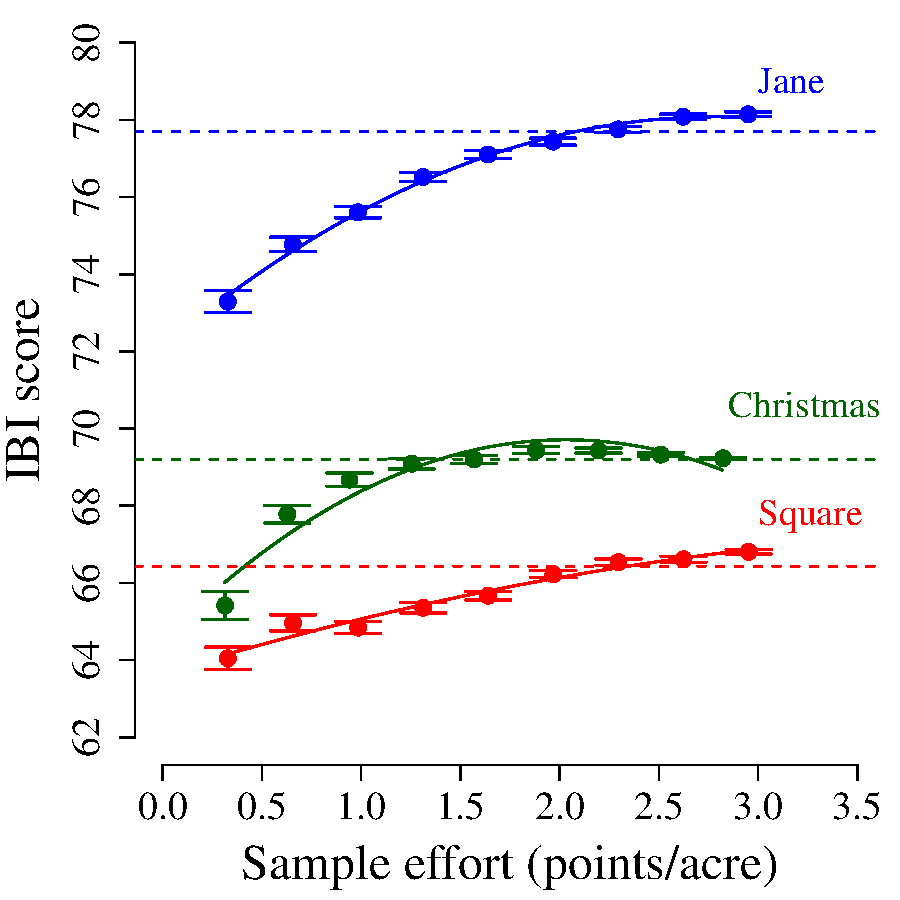
\includegraphics[width=\textwidth]{fig/Beck_GEDsem-ibi_eff.pdf}
\end{center}
\end{column}
\end{columns}
\end{frame}

%%%%%%
\begin{frame}{\textbf{Case 1: Minnesota lakes}}{\textbf{Evaluating biological response}}
\onslide<+->{How appropriate is the IBI for characterizing effects of multiple stressors? Will it work within an assessment/impairment framework?\\~\\}
\onslide<+->{
\vspace*{-0.1in}
\begin{center}
\scalebox{0.8}{
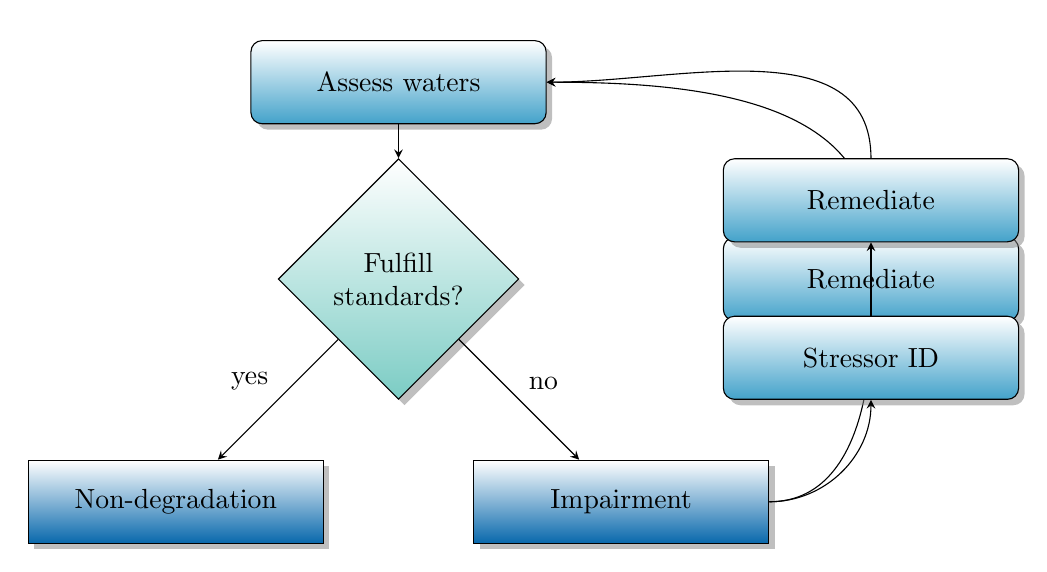
\begin{tikzpicture}[node distance=2.5cm, auto, >=stealth]
	\node[block] (a) {Assess waters};
	\onslide<+->{
	\node[decision] (b)  [below of=a] {Fulfill standards?};
 	\draw[->] (a) -- (b);}
 	\onslide<+->{
 	\node[declare] (c)  [below left of=b, node distance=4cm]  {Non-degradation};
 	\draw[->] (b) -- node[above left] {yes} (c);}
 	\onslide<+->{
 	\node[declare] (d)  [below right of=b, node distance=4cm]  {Impairment};
 	\draw[->] (b) -- node[above right] {no} (d);}
 	\onslide<+>{
 	\node[block] (e)  [right of=b, node distance=6cm]    {Remediate};
 	\draw[->] (d.east) to [out=360,in=270] (e.south);
 	\draw[->] (e.north) to [out=90,in=360] (a.east);}
 	\onslide<+->{
 	\node[block] (f)  [below of=e, node distance=1cm]    {Stressor ID};
 	\node[block] (g)  [above of=e, node distance=1cm]    {Remediate};
	\draw[->] (d.east) to [out=360,in=270] (f.south);
	\draw[->] (f.north) to [out=90,in=270] (g.south);
 	\draw[->] (g.north) to [out=90,in=360] (a.east);}
\end{tikzpicture}}
\end{center}}
\end{frame}

%%%%%%
\begin{frame}{\textbf{Case 1: Minnesota lakes}}{\textbf{Evaluating biological response}}
\onslide<+->
Consider an IBI with 12 metrics, each scored 1, 3, or 5\\~\\
How many different combinations of metrics lead to the same score?
\onslide<+->


{\centering 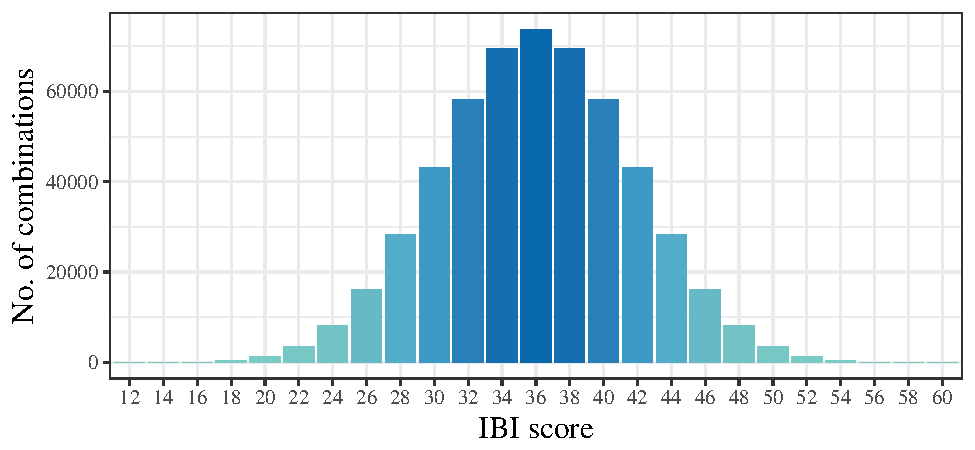
\includegraphics[width=\maxwidth]{fig/ibi_comb-1} 

}



\end{frame}

%%%%%%
\begin{frame}{\textbf{Case 1: Minnesota lakes}}{\textbf{Evaluating biological response}}
\onslide<+->
\textbf{\emph{Develop and implement a framework for evaluating the macrophyte IBI to inform its use in biological monitoring:}} \\~\\
\begin{enumerate}
\onslide<+->
\item How well does the index distinguish between signal and noise? \\~\\
\onslide<+->
\item Can information on stressors and their effects be quantified with certainty? \\~\\
\onslide<+->
\item What stressors primarily influence index response? \\~\\
\onslide<+->
\item How appropriate is a multimetric index for characterizing effects of multiple stressors?
\end{enumerate}
\end{frame}

%%%%%%
\begin{frame}{\textbf{Case 1: Minnesota lakes}}{\textbf{Evaluating biological response}}
\begin{itemize}
\item Dataset of 332 vegetation surveys, courtesy of MNDNR \cite{Beck14a}
\item Numerous covariates describing lake characteristics and anthropogenic stressors
\end{itemize}
\begin{columns}
\begin{column}{0.5\textwidth}
\centerline{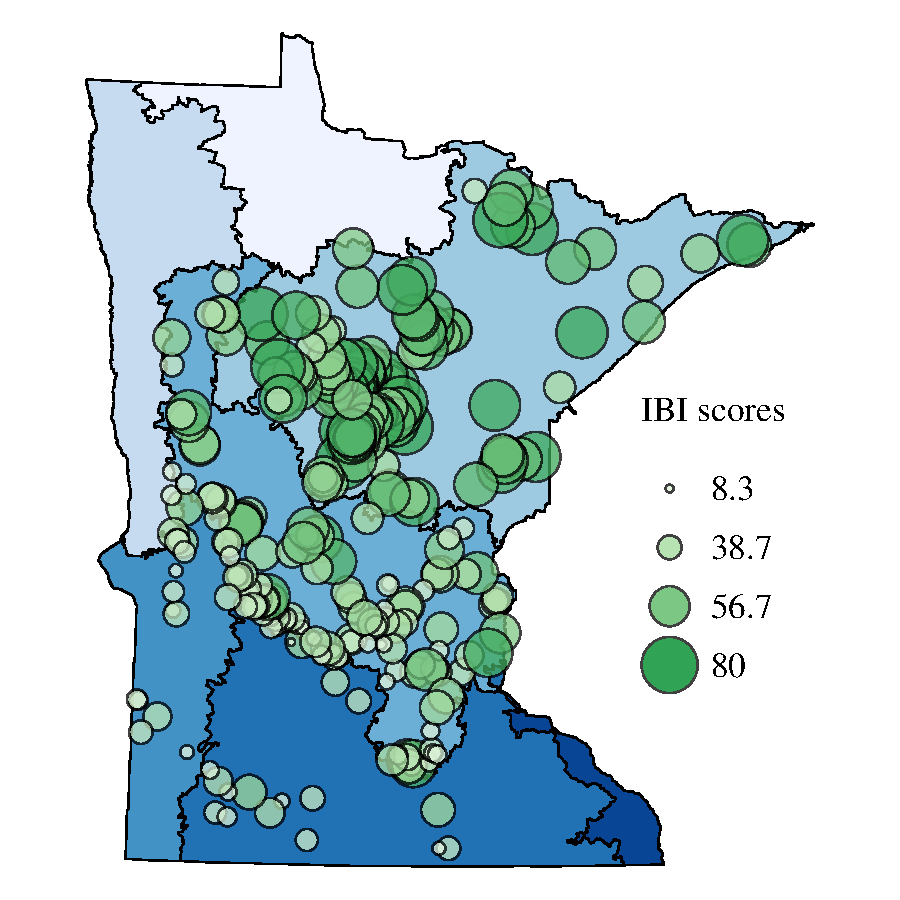
\includegraphics[width=0.9\textwidth]{fig/Beck_GEDsem-ibi_data.pdf}}
\end{column}
\begin{column}{0.5\textwidth}
\scriptsize
\begin{itemize}
\item{lake surface area}
\item{maximum lake depth}
\item{trophic state index}
\item{growing degree days}
\item{percent agriculture in wshed}
\item{percent impervious surfaces in wshed}
\item{density of groundwater wells in wshed}
\item{wshed area to lake area}
\item{crop productivity index of wshed}
\item{dock density}
\item{...}
\end{itemize}
\end{column}
\end{columns}
\end{frame}

%%%%%%
\begin{frame}{\textbf{Case 1: Minnesota lakes}}{\textbf{Evaluating biological response}}
\onslide<+->
Ecological and numerical complexity warrants the use of creative solutions\\~\\
Neural networks to model IBI response\\~\\
\begin{itemize}
\onslide<+->
\item{Essentially a large, non-linear regression model free of assumptions that can handle multivariate response}
\onslide<+->
\item{Models relationships among variables using a network that mimics neuronal structure of the human brain}
\onslide<+->
\item{`Supervised' neural networks are meant for prediction but network information can be used to infer causation}
\end{itemize}
\end{frame}

%%%%%%
\begin{frame}{\textbf{Case 1: Minnesota lakes}}{\textbf{Evaluating biological response}}
\begin{center}
\animategraphics[controls, width =.65\linewidth]{12}{fig/Rplot}{}{} %frame rate is 12 per/sec
\end{center}
\end{frame}

%%%%%%
\begin{frame}{\textbf{Case 1: Minnesota lakes}}{\textbf{Evaluating biological response}}
Modification of Garson's algorithm to determine relative importance of variables [Beck, in press]
\begin{columns}
\begin{column}{0.5\textwidth}
\begin{center}
\includegraphics<1->[width=\textwidth,page=2]{fig/Beck_GEDsem-nnet_relimp1.pdf}
\end{center}
\end{column}
\begin{column}{0.5\textwidth}
\begin{center}
\includegraphics<1>[width=\textwidth,page=11]{fig/Beck_GEDsem-nnet_relimp2.pdf}
\includegraphics<2>[width=\textwidth,page=12]{fig/Beck_GEDsem-nnet_relimp2.pdf}
\includegraphics<3>[width=\textwidth,page=13]{fig/Beck_GEDsem-nnet_relimp2.pdf}
\includegraphics<4>[width=\textwidth,page=14]{fig/Beck_GEDsem-nnet_relimp2.pdf}
\includegraphics<5>[width=\textwidth,page=15]{fig/Beck_GEDsem-nnet_relimp2.pdf}
\includegraphics<6>[width=\textwidth,page=16]{fig/Beck_GEDsem-nnet_relimp2.pdf}
\includegraphics<7>[width=\textwidth,page=17]{fig/Beck_GEDsem-nnet_relimp2.pdf}
\includegraphics<8>[width=\textwidth,page=18]{fig/Beck_GEDsem-nnet_relimp2.pdf}
\includegraphics<9>[width=\textwidth,page=19]{fig/Beck_GEDsem-nnet_relimp2.pdf}
\includegraphics<10->[width=\textwidth,page=20]{fig/Beck_GEDsem-nnet_relimp2.pdf}
\end{center}
\end{column}
\end{columns}
\onslide<11>
Relative importance is summation of product of weights between layers
\end{frame}

%%%%%%
\begin{frame}{\textbf{Case 1: Minnesota lakes}}{\textbf{Evaluating biological response}}
\begin{center}
\begin{figure}[p]
\subfloat[IBI scores]{
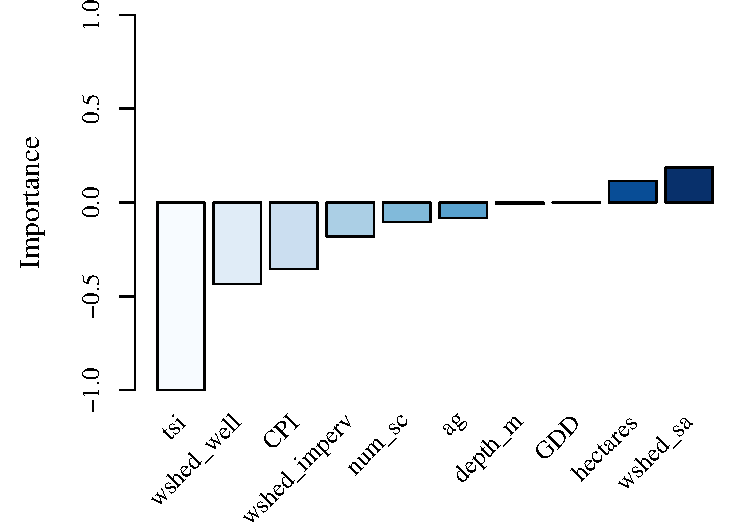
\includegraphics[width=0.5\textwidth,keepaspectratio=T,page=1]{fig/Beck_GEDsem-gar_exp_met.pdf}
}
\subfloat[MAXD metric]{
\includegraphics[width=0.5\textwidth,keepaspectratio=T,page=2]{fig/Beck_GEDsem-gar_exp_met.pdf}
}
\vspace{0.1in}
\caption{Examples of relative importance of explanatory variables based on weights between layers in optimal neural networks.}  
\end{figure}
\end{center}
\end{frame}

%%%%%%
\begin{frame}{\textbf{Case 1: Minnesota lakes}}{\textbf{Evaluating biological response}}
\onslide<+->
Neural networks are powerful enough to model noise in the data \\~\\
The model may be specific to peculiarities the training dataset \\~\\
Uncertainty of variable importance must be quantified - bootstrap! 
\onslide<+->
\begin{center}
\begin{figure}[t]
\subfloat{
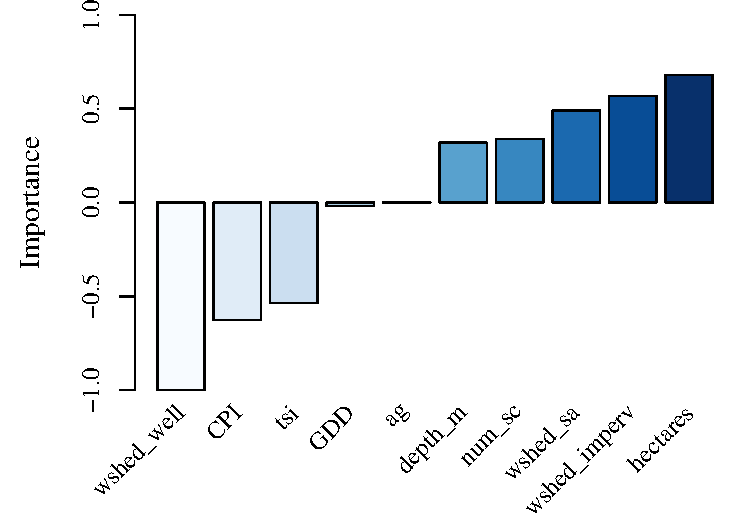
\includegraphics[width=0.5\textwidth,keepaspectratio=T,page=1]{fig/Beck_GEDsem-gar_boot.pdf}
}
\subfloat{
\includegraphics[width=0.5\textwidth,keepaspectratio=T,page=2]{fig/Beck_GEDsem-gar_boot.pdf}
}
\end{figure} %TAXA
\end{center}
\end{frame}

%%%%%%
\begin{frame}{\textbf{Case 1: Minnesota lakes}}{\textbf{Evaluating biological response}}
Lots of uncertainty associated with input contributions... \\~\\
\begin{itemize}
\item One of ten relationships for IBI scores with explanatory variables
\item Four of 80 relationships for metrics with explanatory variables
\pause
\item IBI negatively related to lake trophic state
\item MAXD, OVER, and TAXA negatively related to lake trophic state
\item TAXA positively related to lake size\\~\\
\end{itemize}
\pause
What is the source of this uncertainty? Sample sizes, method, neural network?
\end{frame}

%%%%%%
\begin{frame}{\textbf{Case 1: Minnesota lakes}}{\textbf{Evaluating biological response}}
Potentially competing objectives of an IBI: certainty vs simplicity \\~\\
\pause
\begin{quote}
IBI relies on multiparameters, a requirement when the system to be evaluated is complex. \cite{Karr86} \\~\\
\end{quote}
\begin{quote}
The resulting index allows people without specialized expertise to describe overall condition and to make informed decisions that will affect the health of those resources. \cite{Karr99} \\~\\
\end{quote}
\pause
\begin{quote}
Combining responses into an index hides the component responses, thereby obscuring causation. \cite{Suter93}
\end{quote}
\end{frame}

%%%%%%
\begin{frame}{\textbf{Case 2: Florida estuaries}}{\textbf{Evaluating long-term water quality datasets}}
USEPA Gulf Ecology Division - guidance to Florida DEP and others on criteria development for coastal areas\\~\\
\centerline{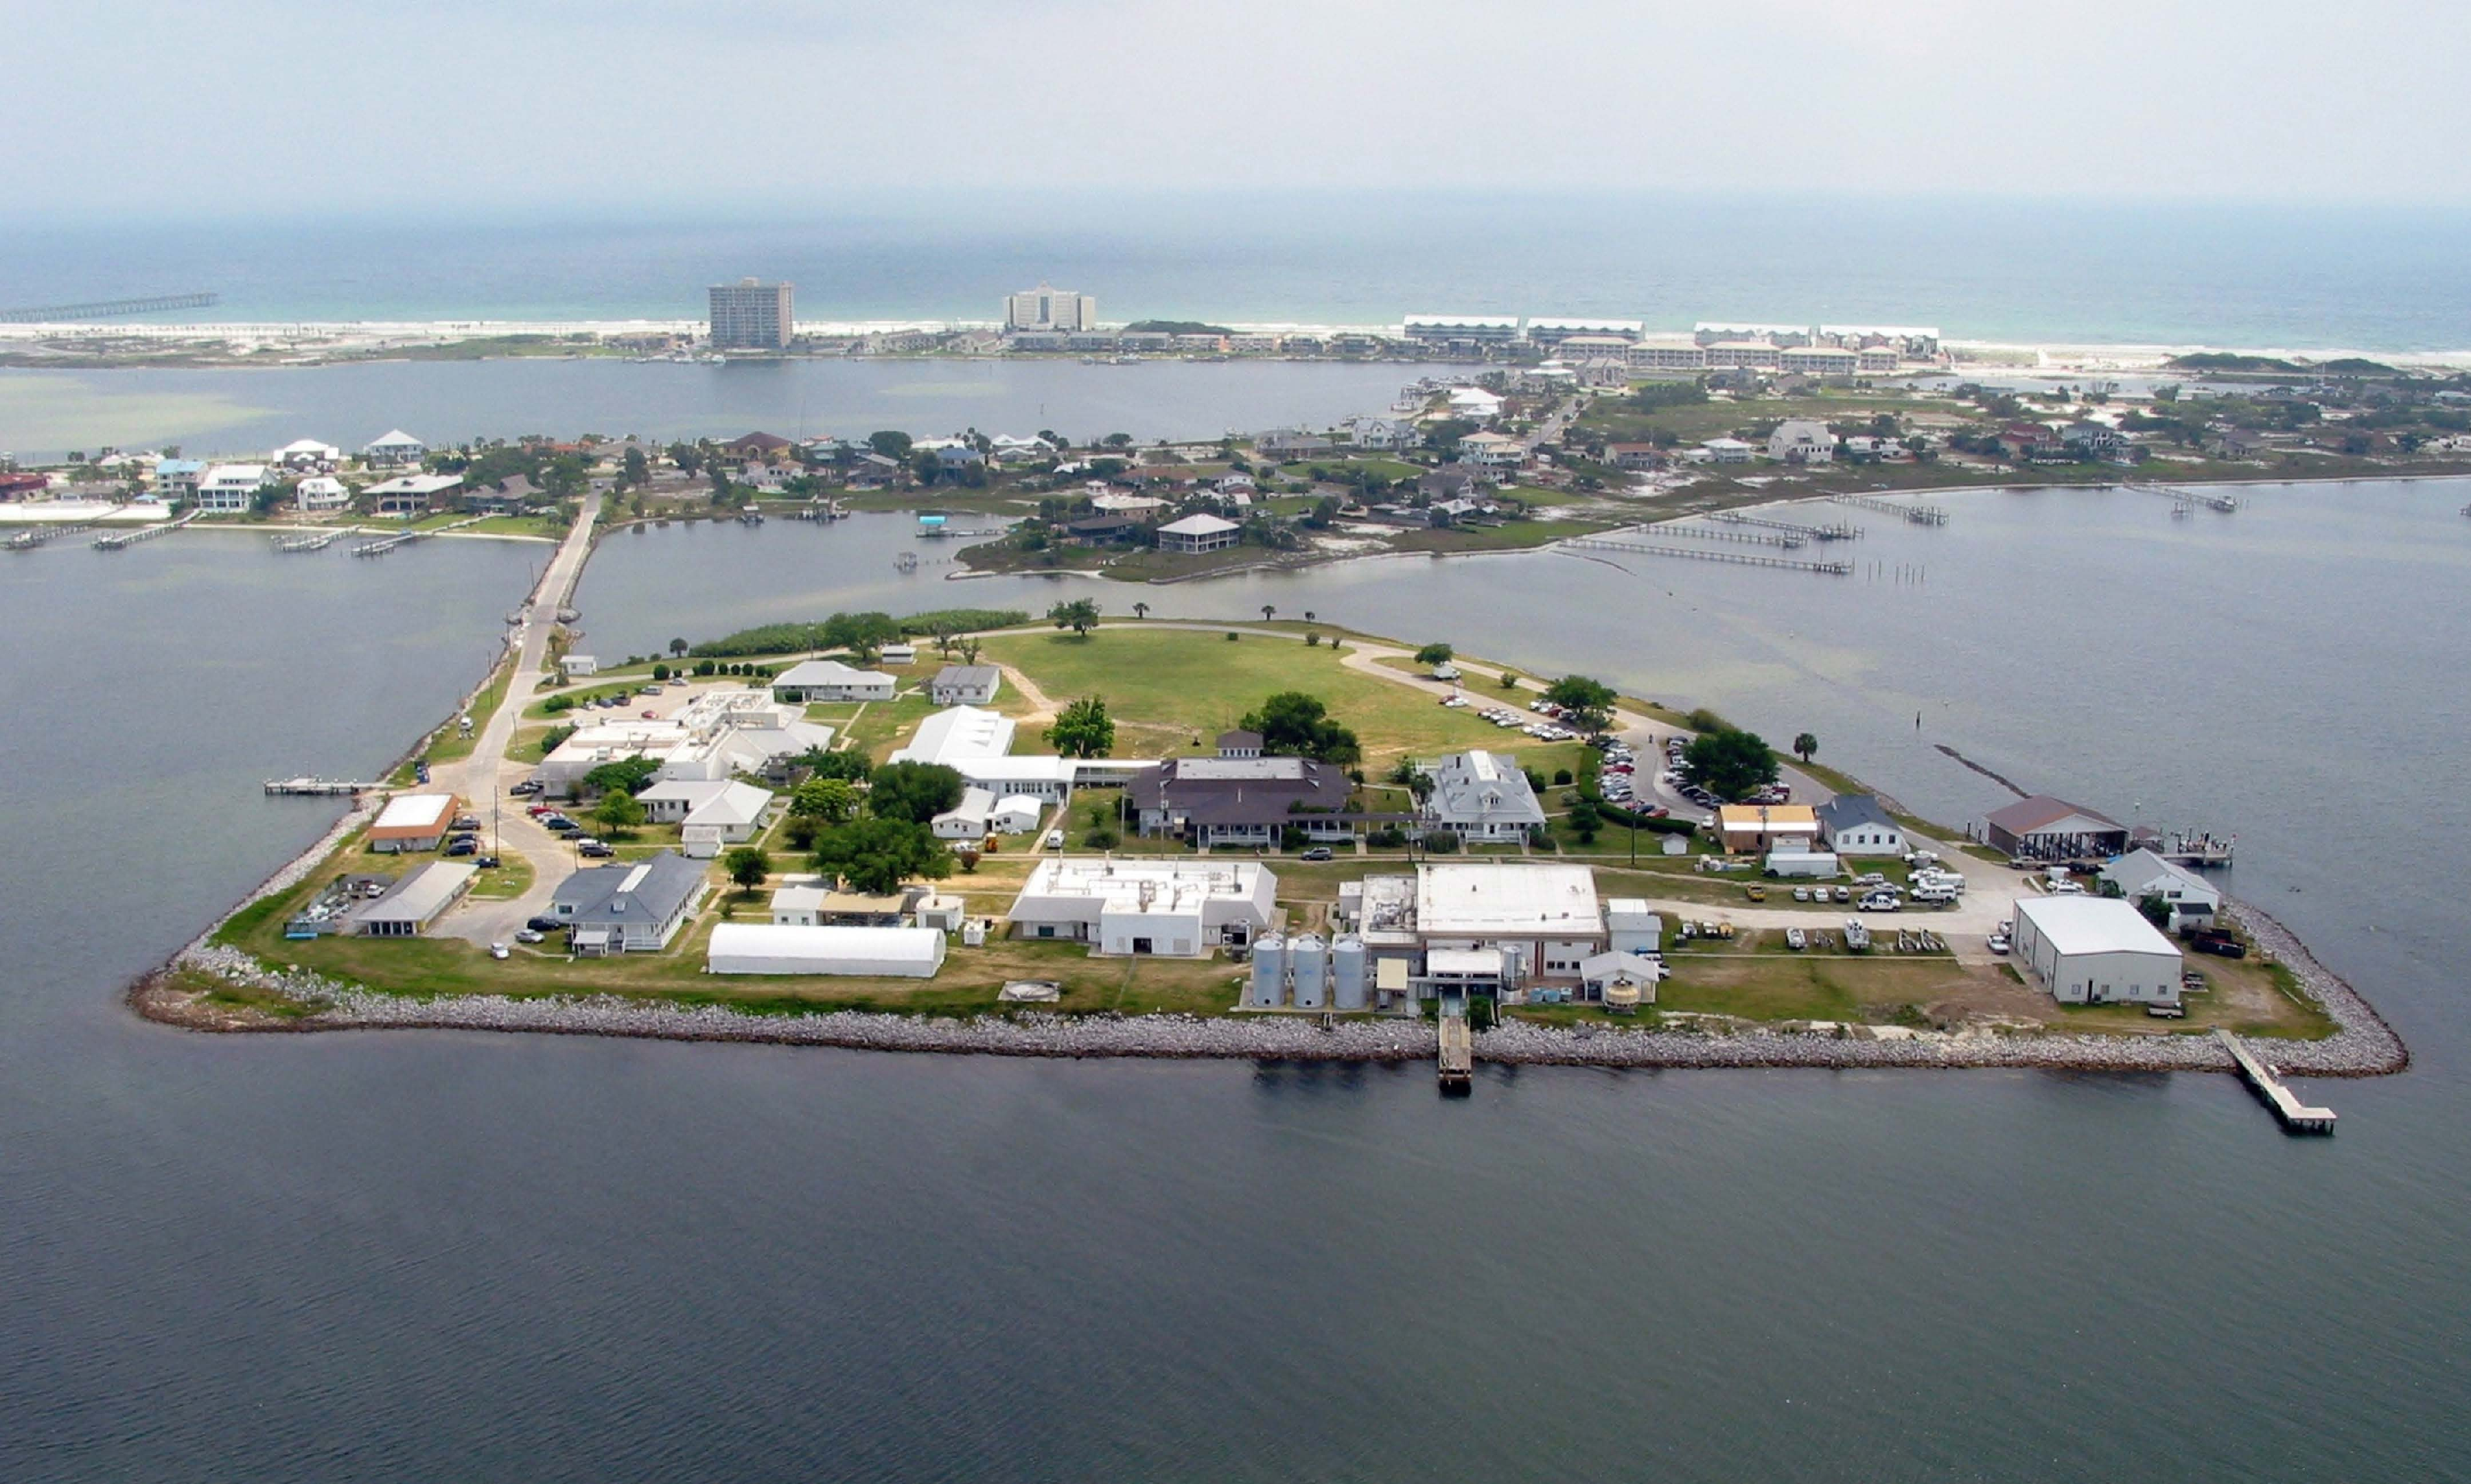
\includegraphics[width = 0.8\textwidth]{fig/sabine.pdf}}
\end{frame}

\section{Case 2: Florida Estuaries}

% tampa bay map, w/ inset


%%%%%%
\begin{frame}{\textbf{Case 2: Florida estuaries}}{\textbf{Evaluating long-term water quality datasets}}
\begin{columns}
\begin{column}{0.5\textwidth}
\begin{itemize}
\item Four bay segments\\~\\
\item Monthly wq data at 50 stations from 1974 to present \\~\\
\item Longitudinal profile of nutrient load and salinity \\~\\
\end{itemize}
\vspace{0cm}\hspace*{15pt}\scalebox{0.7}{\hbox{\tiny Data from \cite{TBEP11}}}
\end{column}
\begin{column}{0.5\textwidth}
\centerline{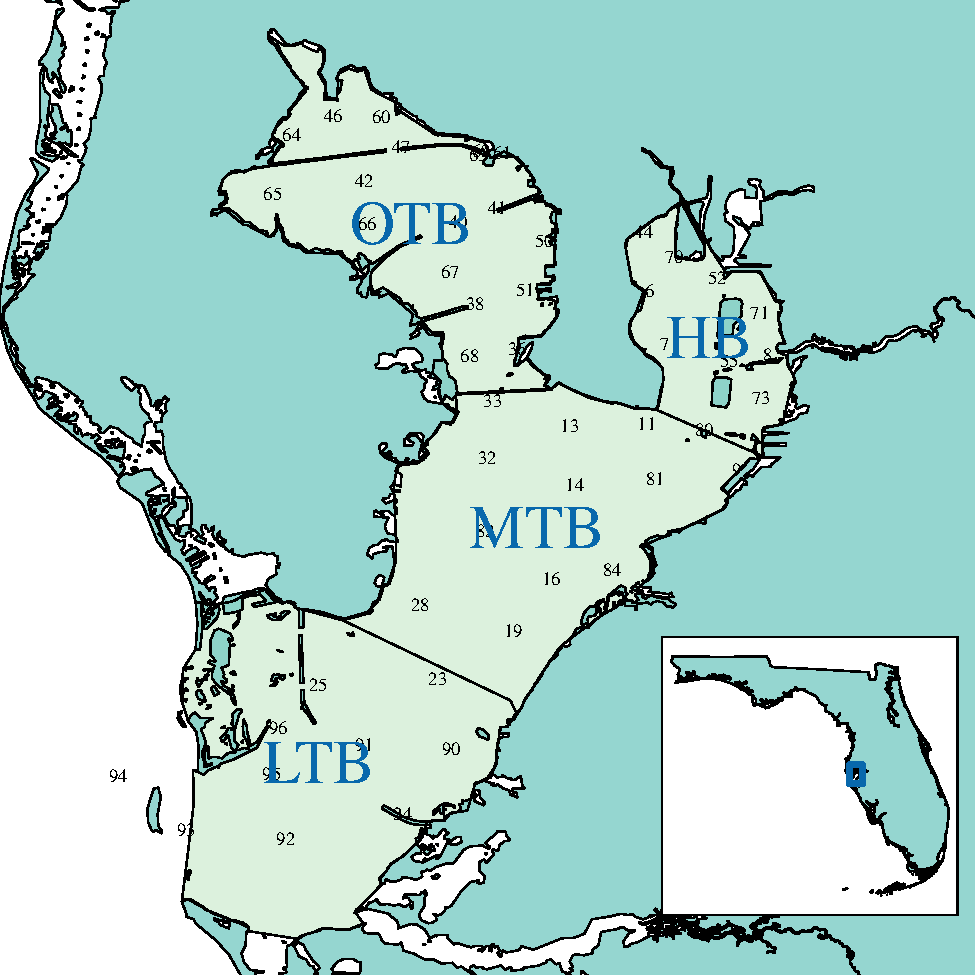
\includegraphics[width = \textwidth]{fig/tb_map.pdf}}
\end{column}
\end{columns}
\end{frame}

%%%%%%
\begin{frame}{\textbf{Case 2: Florida estuaries}}{\textbf{Evaluating long-term water quality datasets}}
\begin{figure}[!ht]

{\centering 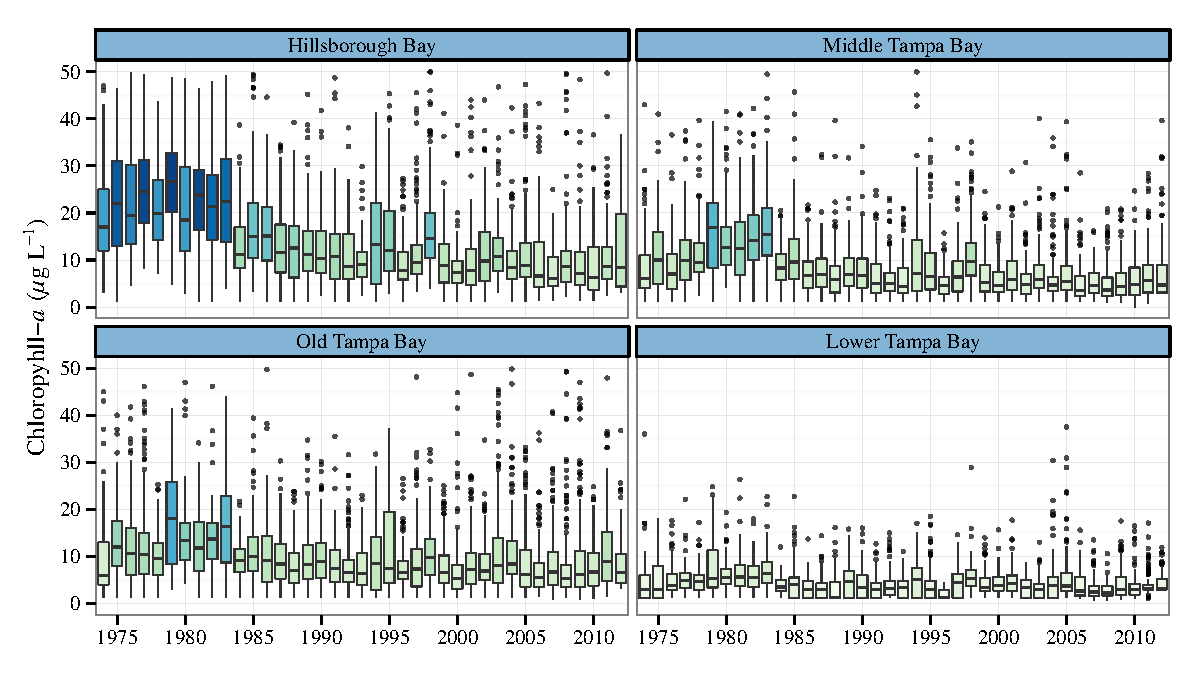
\includegraphics[width=\linewidth]{fig/annual_chl-1} 

}

\caption[Annual trends in chlorophyll for each bay segment]{Annual trends in chlorophyll for each bay segment.}\label{fig:annual_chl}
\end{figure}


\end{frame}

% variation in chl by year, season, and management

%%%%%%
\begin{frame}{\textbf{Case 2: Florida estuaries}}{\textbf{Evaluating long-term water quality datasets}}
What affects our interpretation of chlorophyll response to nutrients?
\vspace{-0.1in}
\captionsetup[subfloat]{captionskip=0pt, position=top}
\begin{figure}
\centering
\subfloat[]{
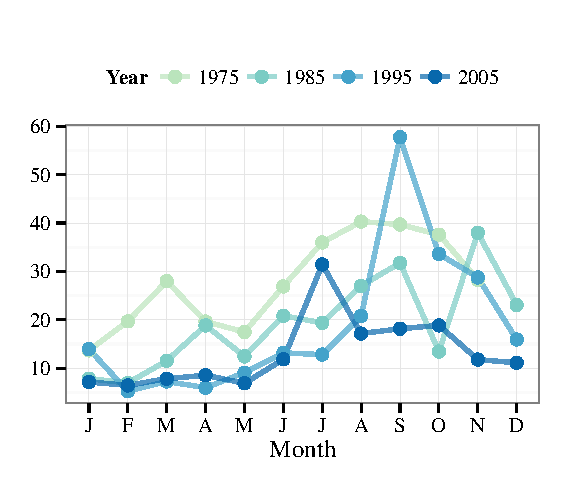
\includegraphics[width=0.46\textwidth,page=1,trim=0.2in 0in 0in 0.35in,clip]{fig/salmoyr.pdf}
\label{fig:salmoyr1}
}
\subfloat[]{
\includegraphics[width=0.46\textwidth,page=2,trim=0.2in 0in 0in 0.35in,clip]{fig/salmoyr.pdf}
\label{fig:salmoyr2}
}

\leavevmode\smash{\makebox[0pt]{\hspace{0em}% HORIZONTAL POSITION           
  \rotatebox[origin=l]{90}{\hspace{3em}% VERTICAL POSITION
    {\color{black} Chlorophyll-\textit{a}}}}}
    \hspace{0pt plus 1filll}\null

\caption{Variation in chlorophyll by {\color{mypal5}\protect\subref{fig:salmoyr1}} time and {\color{mypal5}\protect\subref{fig:salmoyr2}} salinity and management in Hillsborough Bay.  Panel {\color{mypal5}\protect\subref{fig:salmoyr1}} is colored before and after wastewater treatment in 1979.}
\label{fig:salmoyr}
\end{figure}
\captionsetup[subfloat]{position=top}
\end{frame}

%%%%%%
\begin{frame}{\textbf{Case 2: Florida estuaries}}{\textbf{Evaluating long-term water quality datasets}}
\onslide<+->
\begin{block}{Study objective}
Adapt and apply a nutrient response model for estuaries that leverages the descriptive capabilities of large datasets \scriptsize \cite{Beck15}
\end{block}
\vspace{0.2in}
\onslide<+->
Questions of concern -- Can we...
\begin{itemize}
\item ...provide a natural history of water quality that is temporally consistent with drivers of change?
\onslide<+->
\item ...characterize changes in extreme events in addition to describing the mean response?  
\onslide<+->
\item ...improve our understanding of the nutrient-response paradigm in estuaries?
\end{itemize}
\end{frame}

%%%%%%
\begin{frame}{\textbf{Case 2: Florida estuaries}}{\textbf{Evaluating long-term water quality datasets}}
\onslide<+->
\textbf{W}eighted \textbf{R}egression on \textbf{T}ime, \textbf{D}ischarge, and \textbf{S}eason \\~\\
\begin{itemize}
\item Describes a time series in the context of these parameters, locally fitted \\~\\
\item Useful to describe long-term trends, ie., multi-decadal time series \\~\\
\item Evaluation of flow-normalized trends, hypothesis generation
\end{itemize}
\onslide<+->
\vspace{0.1in}
Developed by \cite{Hirsch10} for pollutants in stream/rivers\\~\\
Adapted for tidal waters by \cite{Beck15}
\end{frame}



%%%%%%
\begin{frame}[t]{\textbf{Case 2: Florida estuaries}}{\textbf{Evaluating long-term water quality datasets}}
\onslide<1->
How does it work?  
\begin{center}
$\ln\left(N\right) = \beta_0 + \beta_1 t + \beta_2 Sal + \beta_3 \sin\left(2\pi t\right) + \beta_4 \cos\left(2\pi t\right)$\\~\\
$N$: nitrogen (or other response endpoint)\\
$t$: time\\
$Sal$: Salinity (or other flow-related variable)
\end{center}
\includegraphics<2>[width = \textwidth, page = 1]{fig/wrtds_pieces.pdf}
\includegraphics<3>[width = \textwidth, page = 2]{fig/wrtds_pieces.pdf}
\includegraphics<4>[width = \textwidth, page = 3]{fig/wrtds_pieces.pdf}
\includegraphics<5>[width = \textwidth, page = 4]{fig/wrtds_pieces.pdf}
\includegraphics<6>[width = \textwidth, page = 5]{fig/wrtds_pieces.pdf}
\end{frame}

%%%%%%
\begin{frame}[t]{\textbf{Case 2: Florida estuaries}}{\textbf{Evaluating long-term water quality datasets}}
This is not the whole story...
\begin{center}
$\ln\left(N\right) = \beta_0 + \beta_1 t + \beta_2 Sal + \beta_3 \sin\left(2\pi t\right) + \beta_4 \cos\left(2\pi t\right)$
\end{center}
One parameter set to many parameter sets - a moving window regression \\~\\
Within each window, a unique regression is fit, weighted by the local salinity, time, and season \\~\\
Similar to a loess/spline smooth but specific to the effects of these three variables on the response
\end{frame}



%%%%%%
\begin{frame}{\textbf{Case 2: Florida estuaries}}{\textbf{Evaluating long-term water quality datasets}}
How does weighted regression work?
\begin{center}
\animategraphics[controls,width=\linewidth]{12}{fig/wtex}{}{} %frame rate is 12 per/sec
\end{center}
\end{frame}

%%%%%%
\begin{frame}{\textbf{Case 2: Florida estuaries}}{\textbf{Evaluating long-term water quality datasets}}
{\small
\Bigtxt{Points}: observed time series (black are weighted, grey is zero weight)\\
\Bigtxt{Green point}: observation at the center of the regression\\
\Bigtxt{Blue line}: Global model with weights specific to the window\\
\Bigtxt{Red line}: Accumulated WRTDS model
}
\begin{center}
\animategraphics[controls,width=\linewidth]{10}{fig/wrtds_pieces2}{}{} %frame rate is 12 per/sec
\end{center}
\end{frame}



%%%%%%
\begin{frame}{\textbf{Case 2: Florida estuaries}}{\textbf{Evaluating long-term water quality datasets}}
\centerline{RMSE fit for unweighted = 0.58, WRTDS = 0.36}
\begin{center}
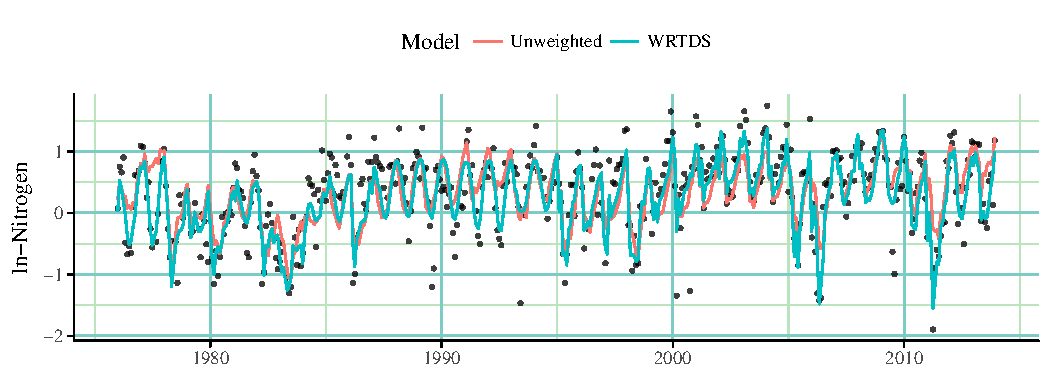
\includegraphics[width = \textwidth]{fig/wrtds_perf.pdf}
\end{center}
\end{frame}

%%%%%%
\begin{frame}{\textbf{Case 2: Florida estuaries}}{\textbf{Evaluating long-term water quality datasets}}
This gives us improved predictions of chlorophyll dynamics...
\begin{figure}[!ht]

{\centering 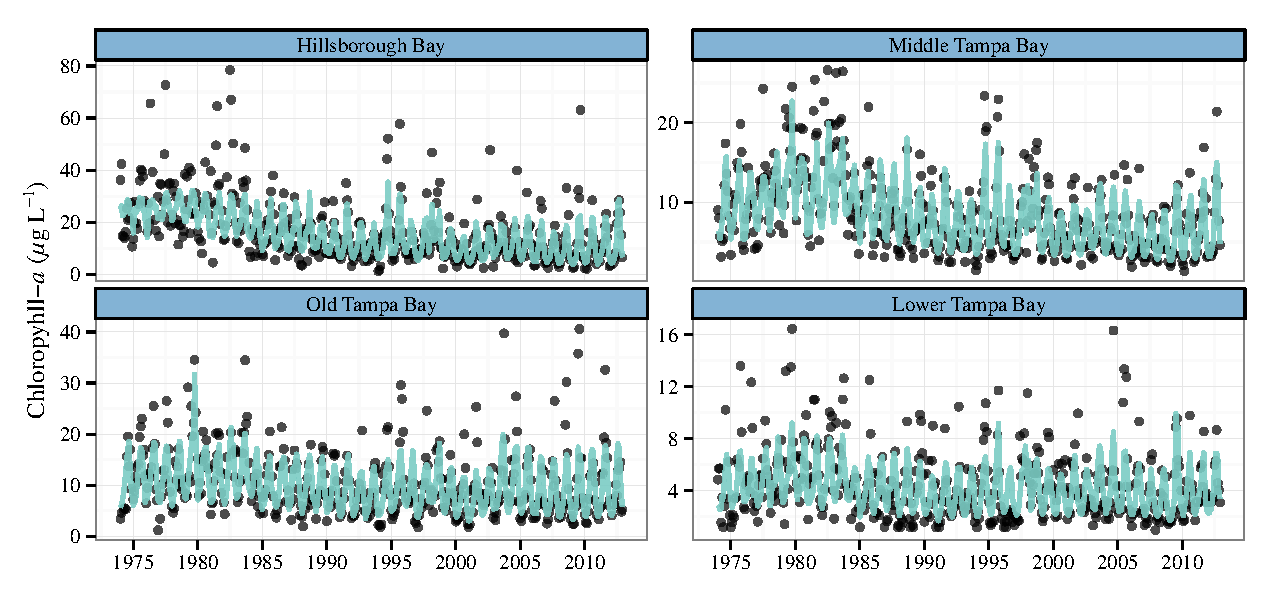
\includegraphics[width=\linewidth]{fig/predvals-1} 

}

\caption[Predicted and observed monthly chlorophyll by segment]{Predicted and observed monthly chlorophyll by segment.}\label{fig:predvals}
\end{figure}


\end{frame}

%%%%%%
\begin{frame}{\textbf{Case 2: Florida estuaries}}{\textbf{Evaluating long-term water quality datasets}}
Because the model is dynamic, we have parameters describing the relationship of chlorophyll with other factors specific to different time periods \\~\\
\begin{columns}[T]
\begin{column}{0.45\textwidth}


{\centering 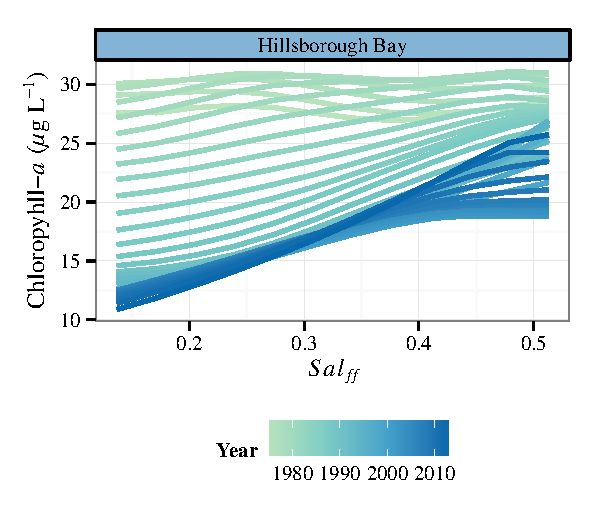
\includegraphics[width=\maxwidth]{fig/hill-1} 

}



\end{column}
\begin{column}{0.45\textwidth}
\begin{itemize}
\item Early period (light blue) - point-sources
\item Late period (dark blue) - non-point sources
\item Chlorophyll shows increasing response to freshwater input in recent years
\end{itemize}
\end{column}
\end{columns}
\end{frame}

% patux trends


%%%%%%
\begin{frame}{\textbf{Application to other systems}}{\textbf{Evaluating long-term water quality datasets}}
Comparing models for trend evaluation \cite{Beck17}
\begin{columns}
\begin{column}{0.38\textwidth}
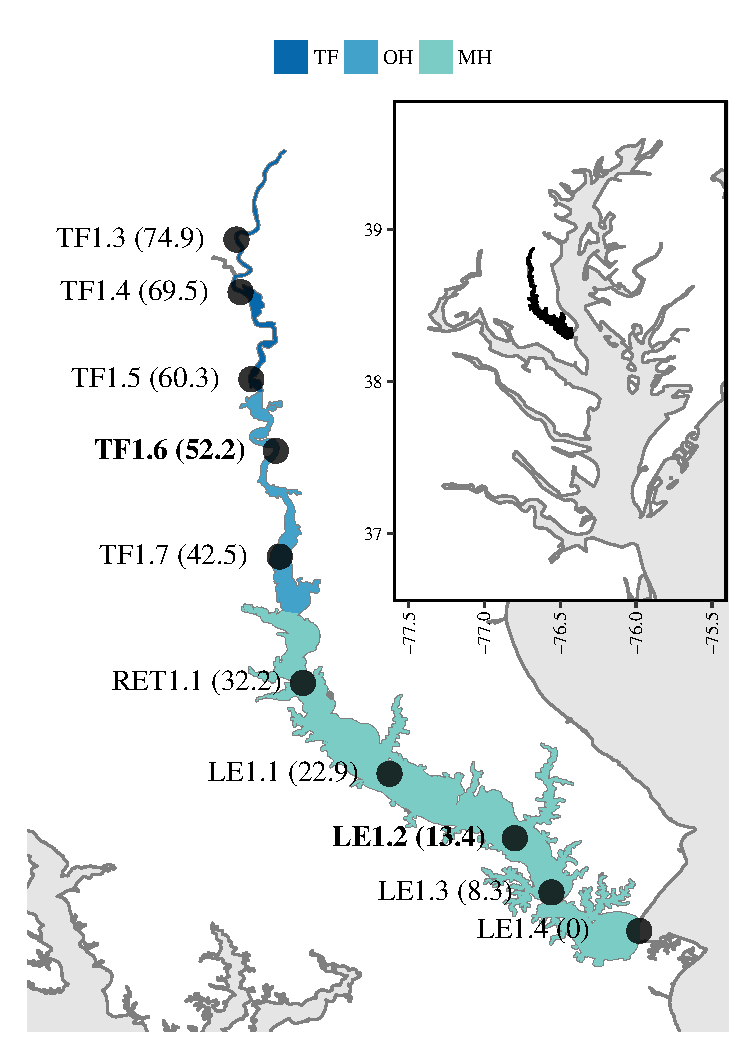
\includegraphics[width = \textwidth]{fig/patux_map.pdf}
\end{column}
\begin{column}{0.65\textwidth}
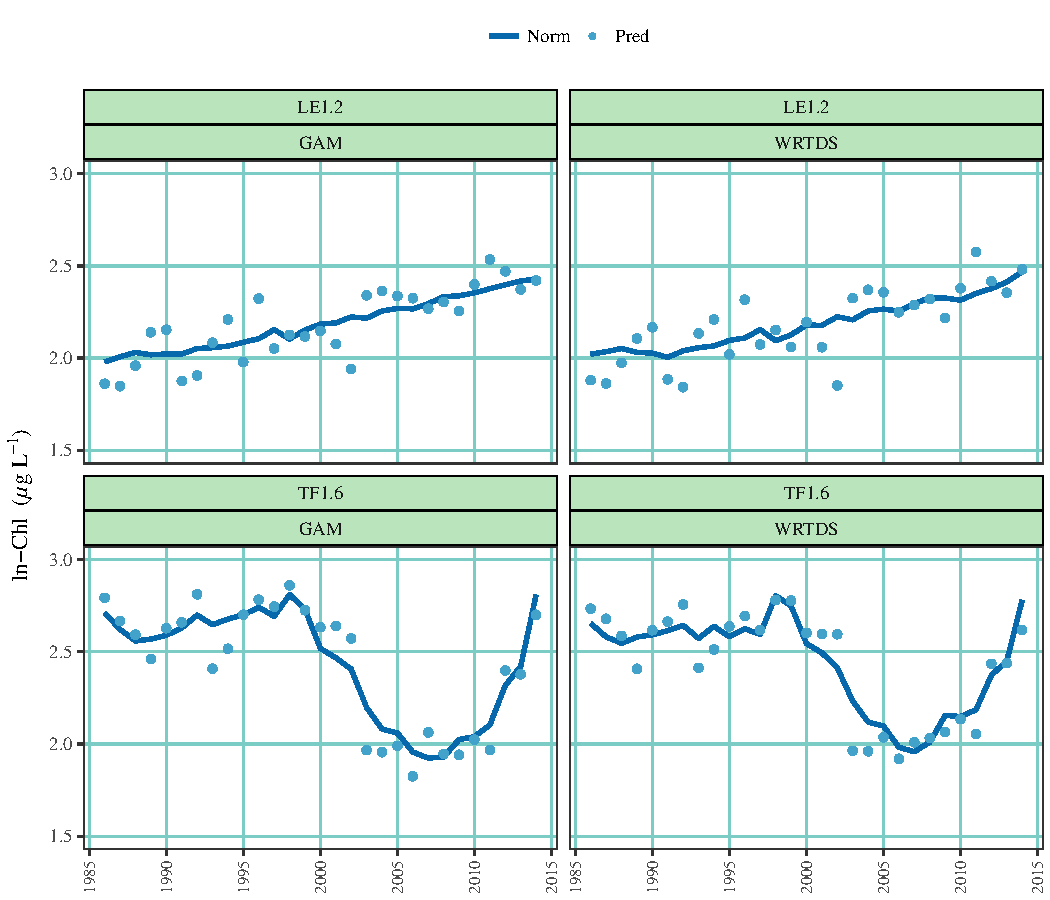
\includegraphics[width = \textwidth]{fig/predann.pdf}
\end{column}
\end{columns}
\end{frame}

%%%%%%
\begin{frame}{\textbf{Application to other systems}}{\textbf{Nitrogen dynamics in the Delta - DIN}} 
\centerline{
\includegraphics[width = 0.93\textwidth, page = 2]{fig/trndsperdin.pdf}}
\end{frame}

%%%%%%
\begin{frame}{\textbf{Application to other systems}}{\textbf{Nitrogen dynamics in the Delta - ammonium}} 
\centerline{
\includegraphics[width = 0.93\textwidth, page = 2]{fig/trndspernh.pdf}}
\end{frame}

%%%%%%
\begin{frame}{\textbf{Application to other systems}}{\textbf{Nitrogen dynamics in the Delta - nitrite/nitate}} 
\centerline{
\includegraphics[width = 0.93\textwidth, page = 2]{fig/trndsperno23.pdf}}
\end{frame}



%%%%%%
\begin{frame}[t]{\textbf{Conclusions}}
\onslide<+->
What does this mean for Tampa Bay and elsewhere?\\~\\
\vspace{-0.2in}
\begin{itemize}
\item Better description of biological endpoints can change conclusions
\end{itemize}
\onslide<+->
\centerline{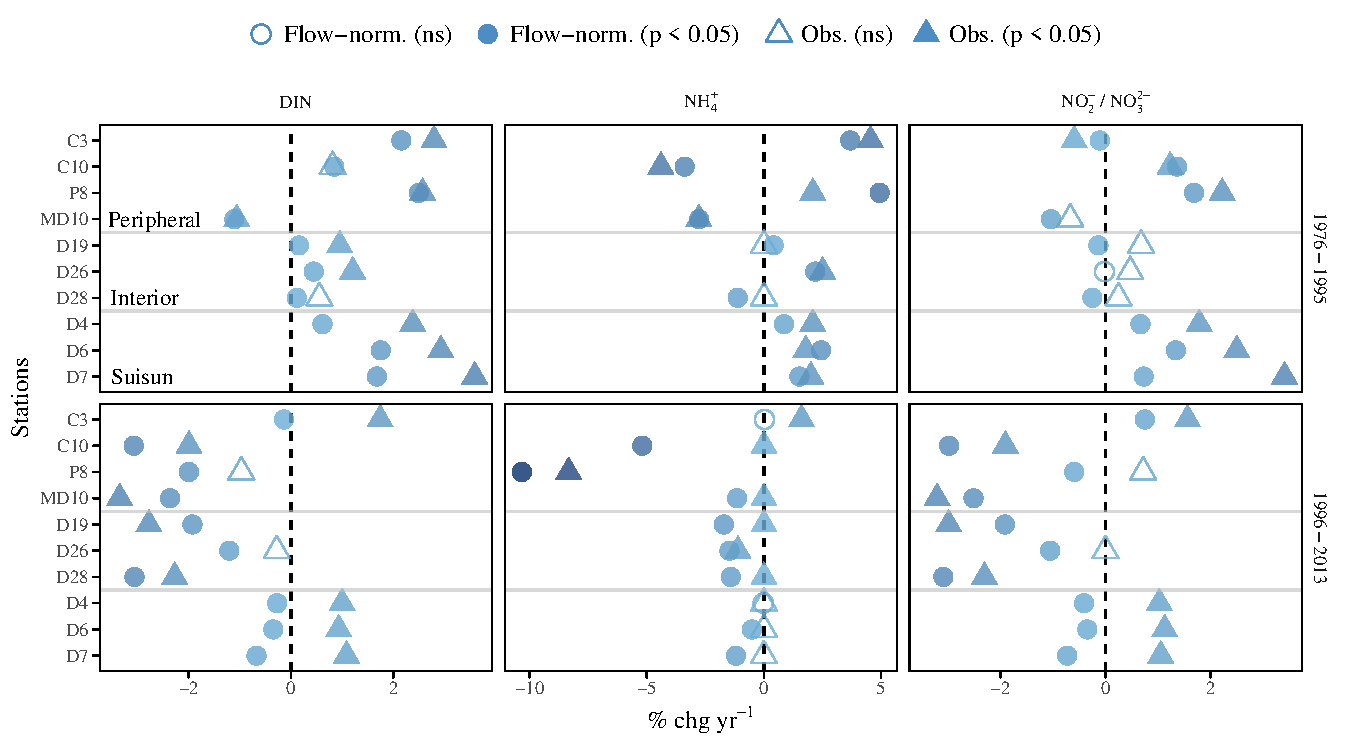
\includegraphics[width = \textwidth]{fig/trndcomp1.pdf}}
\end{frame}

%%%%%%
\begin{frame}[t]{\textbf{Conclusions}}
\onslide<+->
What does this mean for Tampa Bay and elsewhere?\\~\\
\vspace{-0.2in}
\begin{itemize}
\item More detailed evaluation of trends allows greater insight into drivers of change\\~\\
\end{itemize}
\onslide<+->
The model parameters show us a picture...
\centerline{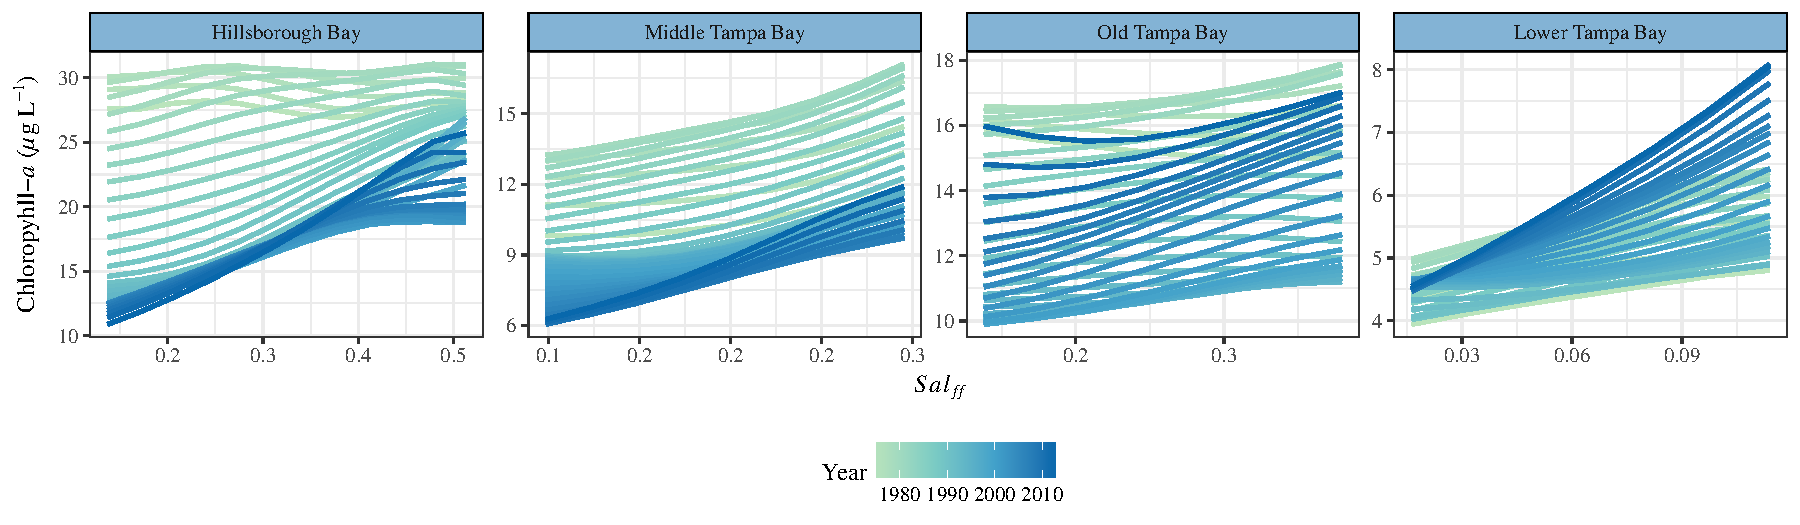
\includegraphics[width = \textwidth]{fig/title_plo.pdf}}
\end{frame}

%%%%%%
\begin{frame}{\textbf{Conclusions}}
\onslide<+->
Observational data are not particularly telling... \\
...so we use \emtxt{indicators} and \emtxt{quantitative methods} to \emtxt{decompose} the observations \\~\\
\onslide<+->
Chosen method depends on the question \\~\\
\onslide<+->
\begin{itemize}
\item More complete description of trends
\item Better link to causal events
\item More comprehensive evaluation of site-specific issues
\item Deconstruct the past to predict the future\\~\\
\end{itemize}
\end{frame}

%%%%%%
\begin{frame}
Acknowledgments:\\~\\
\begin{columns}
\begin{column}{0.8\textwidth}
{\footnotesize
Dissertation committee and advisors: B. Vondracek, L. Hatch, D. Pereira, S. Weisberg \\~\\
Research staff and employees at USEPA Gulf Ecology Division - especially J. Hagy, M. Murrell\\~\\
Field staff and data managers at Hillsborough County Environmental Protection Commission\\~\\
Research staff and employees at the San Francisco Estuary Institute}\\~\\
\end{column}
\begin{column}{0.2\textwidth}
\end{column}
\end{columns}
\vfill
Funding sources and contact:\\~\\
\begin{columns}
\begin{column}{0.4\textwidth}
\centerline{
\includegraphics[width=0.4\linewidth]{fig/epa_logo.png}}
\end{column}
\begin{column}{0.6\textwidth}
\scriptsize
\href{mailto:beck.marcus@epa.gov}{beck.marcus@epa.gov}, 8509342480 \\~\\

\includegraphics[width = 0.05\textwidth]{fig/wordpress.png} Blog: \href{https://beckmw.wordpress.com/}{https://beckmw.wordpress.com/} \\~\\

\includegraphics[width = 0.05\textwidth]{fig/git.png} GitHub: \href{https://github.com/fawda123}{https://github.com/fawda123}\\~\\

\includegraphics[width = 0.05\textwidth]{fig/twitter.png} Twitter: @fawda123
\end{column}
\end{columns}
\vspace{0.2in}
\end{frame}

%%%%%%
\section{References}
\begin{frame}[allowframebreaks,t]{\textbf{References}}
\tiny
\setbeamertemplate{bibliography item}{}
\bibliographystyle{apalike_mine}
\bibliography{refs}
\end{frame}

\end{document}
